\section{Punto de Vista de Cooperación de Proceso de Negocio}

El punto de vista de cooperación de proceso de negocio, promueve la identificación y asociación de roles a través de procesos, en otras palabras, es la vinculación existente entre los procesos y los roles, este punto de vista se deriva directamente del punto de vista de proceso de negocio y al identificar estos roles, permite expandir la forma en que se entiende el proyecto, asignando responsables a procesos.

\subsection{Modelo de Cooperación de Proceso de Negocio}
\begin{figure}[h!]
	\centering
	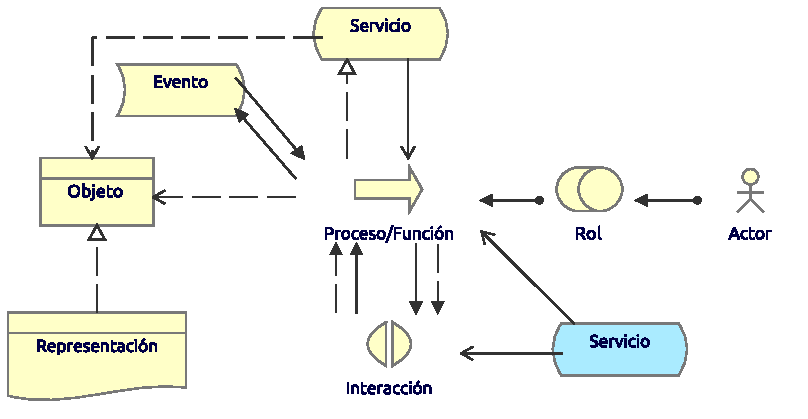
\includegraphics[width=.8\linewidth]{imgs/modelo/ProcesoNegocio}
	\caption{Modelo Cooperación de Proceso de Negocio}
\end{figure}

El modelo del punto de vista de Cooperación de Proceso de Negocio, se compone de un conjunto de partes, principalmente mencionadas en la parte exclusiva del proceso de negocio como lo son: el proceso o función, el evento, los derivados de este evento y proceso como el servicio, el objeto, la interacción y la representación y sin dejar de lado el enlace principal con el proceso el cual es el objetivo, estas partes componen tanto al punto de vista de proceso de negocio como al punto de vista de cooperación de proceso de negocio, a excepción que este segundo punto de vista incluye uno o varios roles, el cual se le asigna al proceso en cuestión.

\clearpage
\subsection{Caso de Cooperación de Proceso de Negocio}
\begin{figure}[h!]
	\centering
	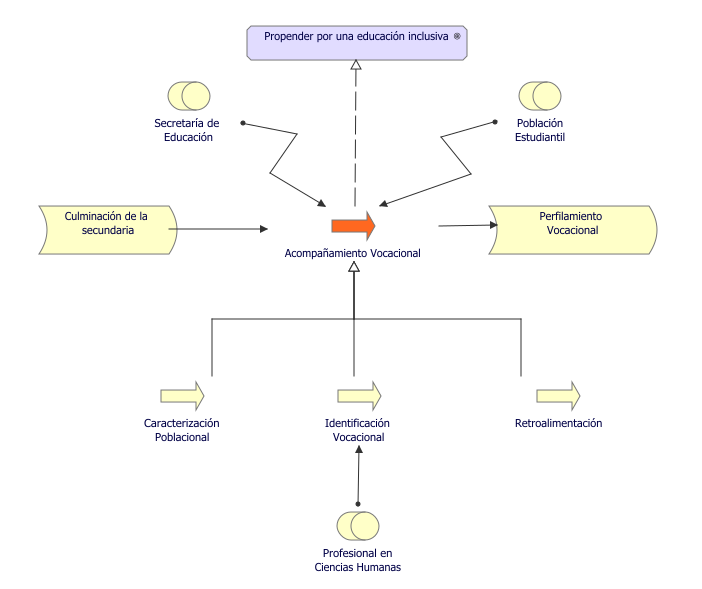
\includegraphics[width=.9\linewidth]{imgs/caso/negocio/CoopProNegocio}
	\caption{Caso Cooperación de Proceso de Negocio}
\end{figure}

Este proyecto de colaboración con el Ministerio de Educación Nacional para tener una educación inclusiva y contribuir con el mejoramiento de la educación en el territorio nacional, posee un gran objetivo el cual es el propender por una educación inclusiva, del cual se deriva el proceso principal de tener un acompañamiento vocacional que lo antecede el evento de negocio de la culminación de la secundaria y lo precede el evento del perfilamiento vocacional, a este gran proceso se le asignan dos roles que intervienen en el, como lo son: la secretaría de educación y la población estudiantil además, este proceso principal cuenta con tres sub procesos: la caracterización poblacional, la identificación vocacional que está vinculada con el rol de los profesionales en ciencias humanas y el subproceso de la retroalimentación.
